
To demonstrate that the $\pi$DTV architecture is practical,
we have built a Digital VCR.
The prototype is implemented on a Pentium II
$450$ MHz Windows $98$ workstation with a Quantum Viking II disk
and $256$ MBytes DRAM.  The main memory and disk are linked
with a SCSI fast bus and managed by an Adaptec AIC-$789x$ based
PCI Ultra2 SCSI controller, both of whom
have much higher data transfer
rates than the disk.           

\begin{figure}[t]
\centerline{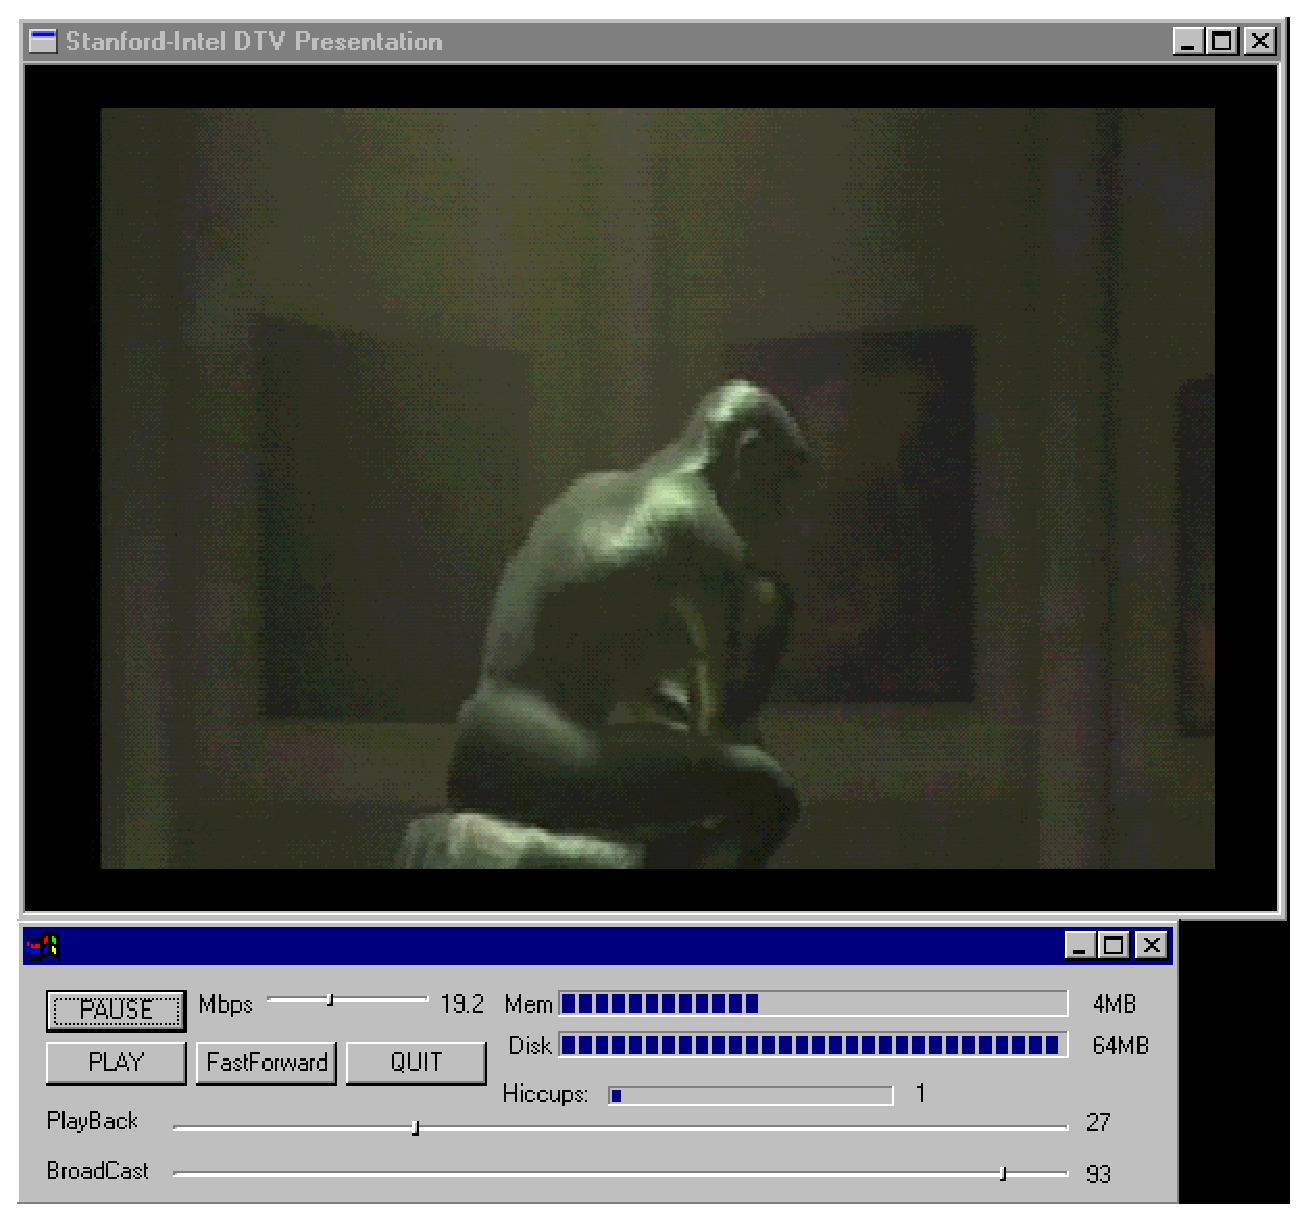
\psfig{figure=digital_vcr.ps,width=240pt,height=200pt}}
\caption{A Digital-VCR Screen Shot.}
\label{fig-codec}
\end{figure}
              
The Digital VCR supports VCR-like interactive functions including
{\em pause}, {\em fast-forward} and {\em instant replay}.
Figure~\ref{fig-codec} shows a screen shot of the user interface
(i.e., {\em codec}) and display. 
At the bottom of the figure is the codec through which a viewer
issues interactive commands and monitors the system.
To issue a command, a viewer selects and presses one
of the control buttons on the upper-left corner of
the codec (described shortly). To monitor the system, the 
codec uses trackbars to display various statuses. The five 
trackbars from the top to the bottom on the codec keep track
of the amount of memory use, the amount of disk use,
the accumulated number of hiccups, the playback progress,
and the broadcast progress.

When a viewer watches a TV program live, memory is
used to buffer the mismatch between the data transmission 
rate and the playback rate. The memory trackbar keeps
track of the current memory use. The disk use
is zero when a program is watched live. When the pause button
is pressed, the excessive data that the DRAM cannot stage is
written onto the disk. Using the disk as a part of the
cache, the VCR can allow the viewer to pause for a substantial amount 
of time (a $9.1$ GBytes disk can buffer more than one hour of
$19.2$ Mbps DTV program).  After returning from the break, the viewer
can press the {\em play} button to resume the playback. At
this time, the decoder consumes data from the disk while the
broadcast data continue arriving and being appended to
the tail of the disk file. The viewer has the option to
perform {\em fast-forward} to catch up with the live 
program. When the fast-forward button is pressed, the Digital VCR
retrieves data from the disk at a faster pace and the decoder
decodes and displays key frames only. The data cached on the disk are
eventually used up and the playback returns to the
live mode. 

